\documentclass[a4paper]{article}

\usepackage[T2A]{fontenc}
\usepackage[russian]{babel}
\usepackage{graphicx}
\usepackage{float}
\usepackage{hyperref}
\usepackage{amsmath, amssymb, diffcoeff, mathtools}
\usepackage{caption}
\usepackage{geometry}
\usepackage{pdfpages}
\usepackage{wrapfig}
\geometry{top=2cm,bottom=2cm,left=2cm,right=2cm}

\newcommand{\minus}{\scalebox{0.75}[1.0]{$-$}}


\date{}

\begin{document}

\begin{center}
\textsc{Санкт-Петербургский национальный исследовательский институт информационных технологий, механики и оптики\\[3mm]
Физический факультет} \\[3mm]

\end{center}
\vspace{5mm}
\line(1,0){\textwidth}
\begin{center}
\textbf{ЛАБОРАТОРНАЯ РАБОТА №2.8\\}
\textbf{"Определение коэффициента вязкости воздуха методом капилляра"}
\end{center}
\vspace{2mm}
\line(1,0){\textwidth}
\vspace{5mm}
\begin{minipage}{0.4\textwidth}
    Группа: Z3144 \\
    Студент: Евгений Турчанин\\
    \vspace{1mm}
\end{minipage}
\hfill
\vspace{1mm}
\line(1,0){\textwidth}

\section{\textbf{Цели работы}}
\begin{enumerate}
	\item Экспериментальная проверка закономерностей движения физического маятника.
    \item Определение вязкости воздуха при комнатной температуре.
\end{enumerate}

\section {\textbf{Задачи}}
Получить зависимость изменения давления в сосуде с течением времени.


\section{\textbf{Теоретическое введение}}

Вязкость (внутреннее трение) – свойство газов и жидкостей
(текучих сред) сопротивляться перемещению одной их части относительно другой. Вязкость проявляется в возникновении сил
внутреннего трения между слоями среды, движущимися друг относительно друга или относительно поверхности твердого тела.
Явление вязкости – одно из явлений переноса, поскольку действующие между слоями силы приводят к переносу импульса
между слоями среды.
На микроскопическом уровне возникновение силы внутреннего трения обусловлено двумя процессами: во-первых, молекулы,
переходя из одного слоя в другой, переносят средний импульс
своего слоя в соседний, во-вторых, на границе между слоями
происходит взаимное выравнивание импульсов молекул за счет
сил межмолекулярного взаимодействия. Первый механизм передачи импульса преобладает в разреженных газах, второй – в
жидкостях.\\
Рассмотрим течение среды в направлении оси $Ox$ (см. Рис.
1) такое, что скорость слоев уменьшается в направлении оси $Oy$. На границе $ab$ между двумя слоями, происходит перенос $х$ проекции импульса частиц среды в направлении оси $Oy$. С макроскопической точки зрения это означает, что на границе слоёв
возникает сила трения $F$, стремящаяся затормозить верхний, более быстрый, слой и ускорить нижний, более медленный. Эта
сила называется силой вязкого (или внутреннего) трения.\\
\begin{wrapfigure}{l}{0.5\textwidth}
  \centering
  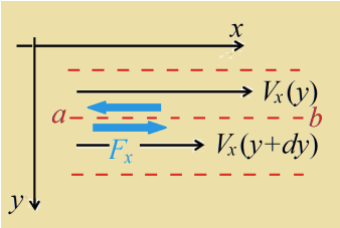
\includegraphics[width=0.48\textwidth]{pick_1}
  \caption{На границе $ab$ между соседними слоями, имеющими разную скорость, действует сила $F_x$ внутреннего трения.}
\end{wrapfigure}
Для многих сред величина силы внутреннего трения $F_x$,
действующая на участке площадью границы между слоями, пропорциональна площади
участка и градиенту скорости
слоев. В этом случае на слой,
лежащий ниже границы $ab$ на
рисунке 1, действует сила
\begin{equation}
    F_x = -\eta \dfrac{\dl V_x}{\dl y}\Delta S
\end{equation}
На слой, лежащий выше
границы, действует такая же по модулю сила, но направленная
противоположно. Коэффициент пропорциональности в формуле
(1) называется коэффициентом динамической вязкости. Этот коэффициент численно равен модулю силы, действующей на единицу площади поверхности каждого из взаимодействующих слоёв,
при градиенте скорости, численно равном единице. В системе СИ
коэффициент динамической вязкости измеряется в · .
Закон вязкого трения (1) был установлен Ньютоном и носит
его имя, а среда, в которой он выполняется, называются ньютоновской жидкостью. Примерами ньютоновской жидкости являются все низкомолекулярные вещества в жидком состоянии и их
гомогенные смеси. Закону (1) подчиняется и течение не сильно разреженных газов\\
Принято подразделять течение по его характеру на ламинарное и турбулентное. Ламинарным называется такое течение, при
котором микрообъемы (частицы) среды движутся по устойчивым
траекториям и среду можно рассматривать как набор слоев движущихся с разными скоростями. Турбулентным (вихревым) течением называется такое, при котором движение частиц среды
становится неустойчивым и хаотичным. Такое течение сопровождается перемешиванием и пульсациями скорости и давления. Для
потока с заданными геометрическими границами по мере достижения достаточно больших скоростей ламинарное течение переходит в турбулентное (см. Приложение 1)\\
При стационарном ламинарном течении ньютоновской несжимаемой жидкости по длинной трубке круглого сечения в ней почти на всём протяжении за исключением небольших областей
вблизи концов устанавливается параболическое распределение скоростей (см. Рис. 2):
\begin{equation}
v(r) = v_0(1-r^2/R^2),
\end{equation}

где $v(r)$ – скорость движения жидкости на расстоянии $r$ от оси
трубки; $v_0$ – скорость на оси трубки; $R$ – радиус трубки.\\
При этом объем жидкости, проходящий в единицу времени
через сечение трубки подчиняется формуле Пуазейля:
\begin{equation}
    \dfrac{\dl V}{\dl t} = \dfrac{\pi R^4}{8 \eta l }(P_1 - P_2),
\end{equation}
Здесь $\dl V$ – объем жидкости, проходящей через сечение трубки
за время $\dl V$; $R$ – радиус трубки; $P_1$, $P_2$ давления в двух сечениях
\begin{figure}[H]
    \begin{center}
    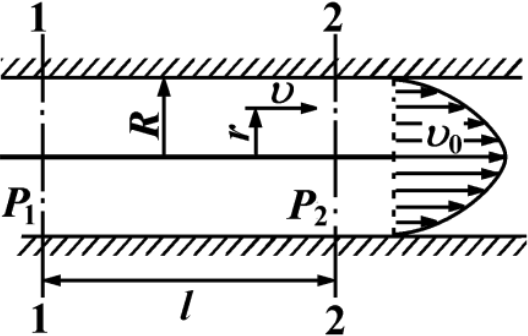
\includegraphics[width=0.48\textwidth]{pick_2}
    \caption{Распределение скорости жидкости в сечении круглой трубки
при ламинарном течении. В соответствии с формулой Пуазейля (2)
объем жидкости протекающей в единицу времени через сечение
трубки определяется отношением разности давлений $P_1$ и $P_2$ в двух
сечениях к расстоянию $l$ между сечениями.}
\end{center}
\end{figure}

трубки, находящихся друг от друга на расстоянии $l$.

В лабораторной работе изучается процесс вытекания воздуха
в атмосферу из большого сосуда (см Рис. 4) через капилляр –
длинную трубку с малым внутренним диаметром ($d$ < 1 мм). В
сосуде с помощью насоса создается избыточное по отношению
к атмосфере давление. После отключения насоса по мере вытекания воздуха давление в сосуде падает. Быстрота вытекания
воздуха и зависимость давления в сосуде от времени зависят от
атмосферного давления $P_a$, объема сосуда $V_c$ , радиуса $R$ капилляра, его длины $L$ и вязкости воздуха $\eta$. Измерение зависимости
давления в сосуде $P_c(t)$ от времени позволяет по известным параметрам установки вычислить вязкость воздуха.\\

Формула (3) выводится в предположении, что среда, текущая
\begin{figure}[H]
    \begin{center}
    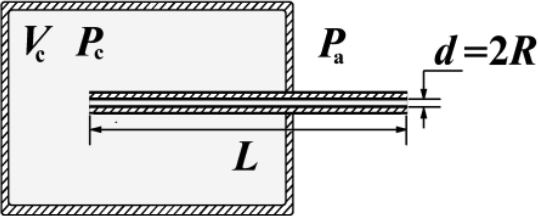
\includegraphics[width=0.48\textwidth]{pick_3}
    \caption{Основная часть лабораторной установки – сосуд достаточно
большого объема $V_c$, в котором создается давление $P_c$ больше, чем
давление $P_a$ в окружающей атмосфере и тонкий капилляр длиной $L$ и
радиусом $R$, соединяющий сосуд с атмосферой.}
\end{center}
\end{figure}

по трубке не сжимаема и имеет плотность, независящую от давления. При течении газа вместе с изменением давления будет
меняться и его плотность, поэтому формула, строго говоря, будет справедлива только для небольших расстояний $l$, на которых
давление и плотность будут меняться незначительно. Если в качестве такого расстояния взять бесконечно малое смещение $\dl x$ 
вдоль трубки, то формула (3) преобразуется к виду

\begin{equation}
\dfrac{\dl V}{\dl t} = \dfrac{\pi R^4}{8\eta}\dfrac{P(x) - P(x+\dl x)}{\dl x} = -\dfrac{\pi R^4}{8\eta}\dfrac{\dl P}{\dl x},
\end{equation}
где $P(x)$ - давление в точке с координатой $x$. Перейдем в этом
уравнении от прошедшнего объема $\dl V$ к перенесенной массе $\dl m$:

\begin{equation}
    \dfrac{\dl m}{\dl t} = \dfrac{p\dl V}{\dl t} = -\dfrac{\pi R^4\rho}{8 \eta} \dfrac{\dl P}{\dl t},
\end{equation}
где $\rho$ - плотность газа.\\
В лабораторной работе изучается течение воздуха при давлениях на несколько десятков процентов превышающих атмосферное. При таких давлениях воздух ведет себя как идеальный
газ, и в состоянии термодинамического равновесия при температуре $T$ для массы $m$ газа выполняется уравнение Менделеева–Клапейрона:
\begin{equation}
    PV = \dfrac{m}{M}RT,
\end{equation}

где $V$ - объём, занимаемый газом, $M$ - молярная масса газа, $R$
- универсальная газовая постоянная. Плотность газа $\rho$ в соответствии с этим уравнением выражается через параметры состояния газа следующим образом

\begin{equation}
    \rho = \dfrac{PM}{RT},
\end{equation}

При дальнейшем рассмотрении будем полагать, что течение газа
происходит достаточно медленно, чтобы формула (7) выполнялась
в каждом сечении капилляра, и уравнение Менделеев-Клапейрона
(6) было справедливо для газа в сосуде в каждый момент времени. Кроме того будем считать температуру газа постоянной.
Тогда плотность газа по уравнению (7) будет пропорциональна
давлению.\\
Теоретически вязкость $\eta$ идеального газа определяется соотношением
\begin{equation}
    \eta = \dfrac{1}{3}V_{\text{ср}}\lambda \rho,
\end{equation}

где $V_{\text{ср}}$ - средняя арифметическая скорость молекул газа; $\lambda$ -
средняя длина свободного пробега молекул. Средняя скорость
молекул зависит только от температуры газа:
\begin{equation}
    V_{\text{ср}} = \sqrt{\dfrac{8RT}{\pi M}},
\end{equation}
и при постоянной температуре не зависит от плотности газа.
Средняя длина свободного пробега молекул газа определяется
концентрации молекул $n$:
\begin{equation}
    \lambda = \dfrac{1}{\sqrt{2}\pi d^2 n },
\end{equation}
и, поскольку концентрация связана с плотностью соотношением: $n = \rho/m_0$, где $m_0$ - масса одной молекулы, из формулы (10)
следует, что средняя длина свободного пробега зависит от плотности обратно пропорционально. Таким образом, при постоянной
температуре в формуле вязкости (8) множитель $V_{\text{ср}}$ не зависит
от плотности, множитель $\lambda$ изменяется обратно пропорционально
плотности. Следовательно, сама вязкость не зависит от плотности.\\
При стационарном течении газа по капилляру масса, переносимая в единицу времени через каждое сечение капилляра должна быть одинакова, т. е. поток массы $\dl m$ 
$\dl t = const$ на всем протяжении капилляра. При этом из-за независимости вязкости от
плотности из формулы (5) следует, что на всем протяжении капилляра $\dfrac{\dl P}{\dl t}\sim \dfrac{1}{\rho}$, или с учетом соотношения (7)

\begin{equation}
    \dfrac{\dl P}{\dl t} \sim \dfrac{1}{P}
\end{equation}
Обозначив коэффициент пропорциональности в этой формуле $K$,
запишем формулу (11) в виде
\begin{equation}
    \dfrac{\dl P}{\dl x} = \dfrac{K}{P}P\dl P = K\dl x
\end{equation}

Чтобы найти выражение для коэффициента $K$, проинтегрируем
второе уравнение (12) от координаты $x_0$ начала капилляра до координаты $x_1=x_0+L$ конца капилляра (см. Рис. 4). Учитывая,
что давление $P(x_0)$ на входе капилляра равно давлению $P_c$ в сосуде, а давление на выходе капилляра $P(x_1)$ равно атмосферному
давлению $P_a$ в результате интегрирования получим

\begin{equation}
    \dfrac{1}{2}\left(P_a^2-P_c^2\right) = KL
\end{equation}
Отсюда
\begin{equation}
    K = -\dfrac{(P_c^2-P_a^2)}{2L}
\end{equation}
Используя написанное выше, найдем соотношение между быстротой изменения давления в сосуде $\dfrac{\dl P_c}{\dl t}$ и текущим значением $P_c$ 
этого давления. Пусть из сосуда за время $\dl t$ выходит масса $\dl m$.
При этом давление газа в соответствие с уравнением (6) изменяется на $\dl P_c = -\dl m RT/(V_cM)$, следовательно:
\begin{equation}
    \dfrac{\dl P_c}{\dl t} = -\dfrac{RT}{V_cM}\dfrac{\dl m}{\dl t}
\end{equation}
Подставим сюда выражение (4), в котором используем первую
формулу (11), выражение (6) для плотности и выражение (14)
для коэффициента $K$. В итоге получим следующее соотношение:
\begin{equation}
    \dfrac{\dl P_c}{\dl t} = -\alpha(P_c^2-P_a^2)
\end{equation}
Коэффициент в этом уравнении зависит от вязкости газа и параметров установки:
\begin{equation}
\alpha = \dfrac{\pi R^4}{16\eta V_cL}
\end{equation}
Разделив переменные в уравнении (16) получим:

\begin{equation}
    \dfrac{\dl P_c}{(P_c^2-P_a^2)}=-\alpha \dl t
\end{equation}
Интегрирование этого уравнения от начального (при $t = 0$) значения давления $P_{c0}$ до значения $P_c$ в некоторый момент времени t дает: 
\begin{equation}
    \dfrac{1}{2P_a}\left[\ln \left(\dfrac{P_c-P_a}{P_c+P_a}\right) - \ln \left(\dfrac{P_{c0-P_a}}{P_{c0}+P_a} \right)\right]=-\alpha t 
\end{equation}
Введем следующие обозначения:

\begin{equation}
    X = \ln \left(\dfrac{P_c-P_a}{P_c+P_a} \right); \; X_0 = \ln\left(\dfrac{P_{c0}-P_{a}}{P_{c0}+P_a} \right); \; C = 2P_a\alpha
\end{equation}

И перепишем уравнение (19) в виде
\begin{equation}
X = X_0 - Ct
\end{equation}
Как видим, зависимость величины $X$ от времени линейная с коэффициентом наклона $'C'$\\
В лабораторной работе измеряется зависимость $P_c(t)$ давления в сосуде от времени. С помощью первой формулы (20) для
каждого значения давления $P_c$ вычисляется величина $X$, тем самым находится зависимость X(t). На основе зависимости X(t)
определяется коэффициент $C$ и по его значению вычисляется
вязкость воздуха. Чтобы получить окончательное выражение для
вязкости, подставим выражение $\alpha$ из формулы (17) в определение коэффициента $C$ (последняя формула (20)) и разрешим
получившееся уравнение относительно вязкости. Таким образом
\begin{equation}
    \eta = \dfrac{\pi R^4 P_a}{8V_cLC}
\end{equation}
Используемый в работе сосуд имеет цилиндрическую форму
и для определения его объема измеряются его высота $H_c$ и диаметр основания $D_c$ ,по которым вычисляется его объем:
\begin{equation}
    V_c = \dfrac{1}{4}\pi D_c^2H_C
\end{equation}



\section{Экспериментальная установка}
\begin{figure}[H]
    \begin{center}
    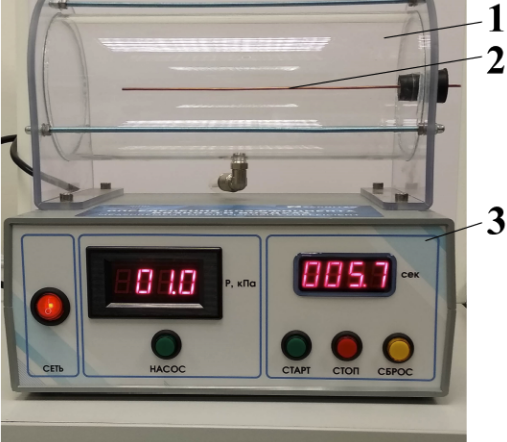
\includegraphics[width=0.48\textwidth]{pick_4}
    \caption{Экспериментальная установка}
\end{center}
\end{figure}

\begin{enumerate}
    \item  Сосуд, в котором создается избыточное давление.
    \item Капилляр, соединяющий сосуд с атмосферой.
    \item Лицевая панель стенда Назначение кнопок и индикаторов, расположенных на лицевой панели следующее: – «СЕТЬ» – кнопка
включения электрического питания стенда; – «Р, кПа» – индикатор значения $\Delta P = P_c-P_a$, разности давлений в сосуде
и в окружающей атмосфере ; – «НАСОС» – кнопка, при нажатом состоянии которой встроенный насос нагнетает воздух в
сосуд; – «сек» – индикатор показаний встроенного секундомера;
– «СТАРТ», «СТОП», «СБРОС» – кнопки запуска, останова и
сброса показаний встроенного секундомера, соответственно
\end{enumerate}


\section{\textbf{Обработка результатов}}

\begin{figure}[H]
    \begin{center}
        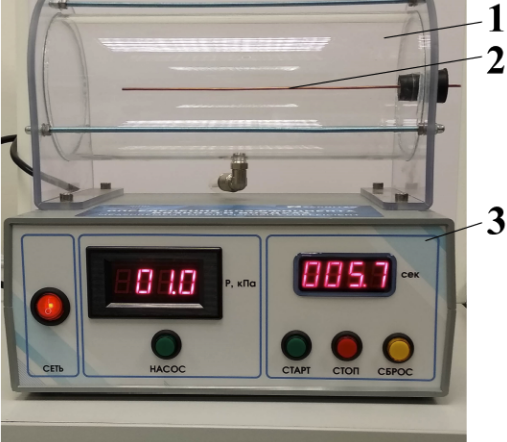
\includegraphics[width=0.48\textwidth]{pick_4}
    \end{center}
\end{figure}

\end{document}
   

